\section{Basic Concept}
\label{sec:concept}

We advocate a concept of ``mobility CPS in the cloud''.
Many mobility CPS applications are often battery-operated, and cannot
accommodate large power consumers unless they equip special battery
facilities.
Integrating cloud technology, however, allows computations and data to be
offloaded over the network and we are freed from power consumption
issues.
For simplicity of description, this paper presents our concept in the
context of autonomous driving, but it is highly applicable for many
other mobility CPS applications.

\begin{figure}[!t]
 \centering
 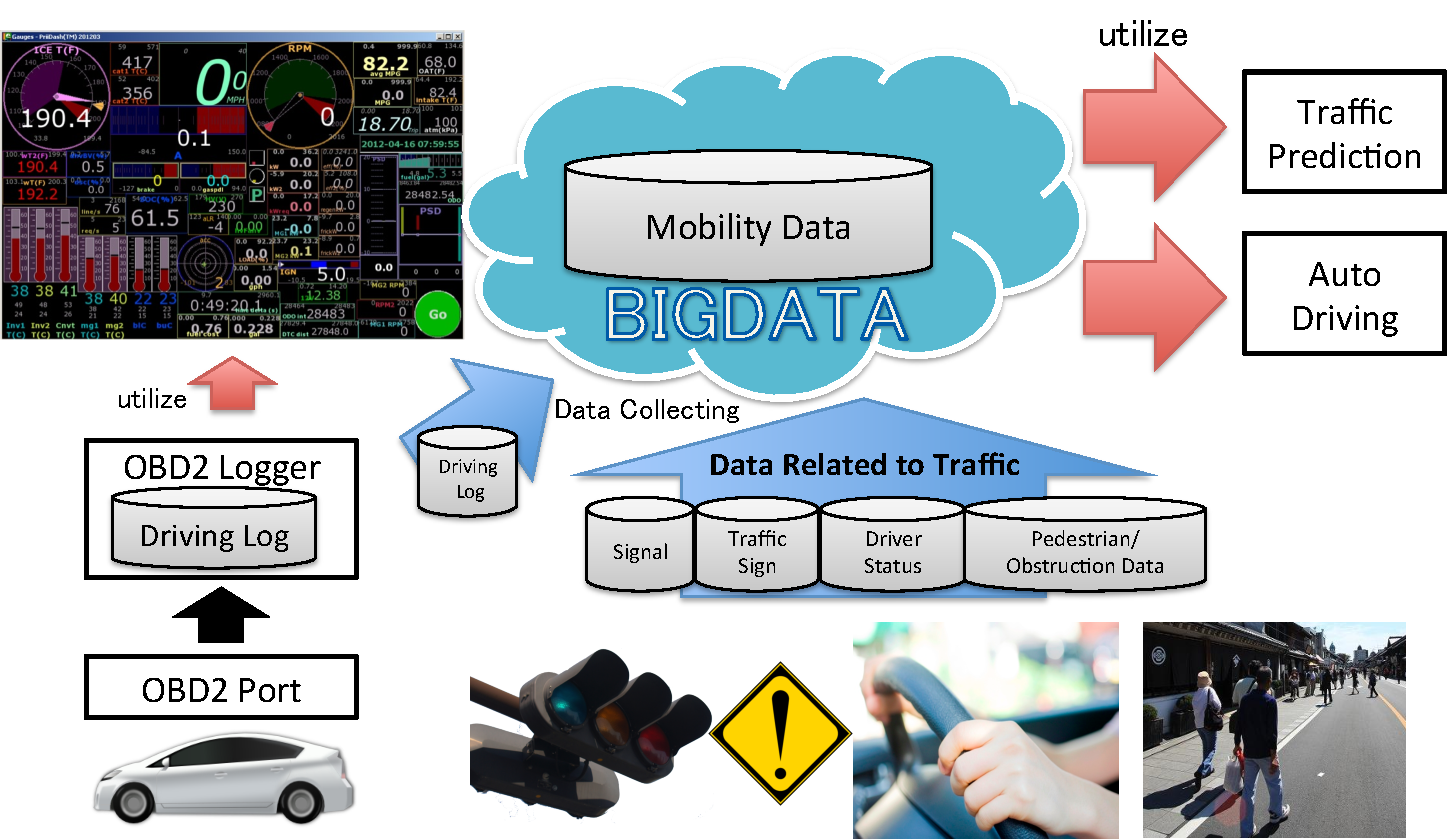
\includegraphics[width=\hsize]{fig/OBD2.pdf}
 \caption{Collecting automotive and environmental data.}
 \label{fig:obd2}
\end{figure}

Grand challenges of mobility CPS include a modeling of the physical
world that underlies a real-time cyber-understanding of the physical
world including environmental perception and motion control.
This modeling of the physical world requires accumulative collection of
real-world data, often referred to as ``Big Data''.
Fig. \ref{fig:obd2} illustrates an example of collecting automotive data
through the on-board diagnosis (OBD) connectors as well as environmental
data.
We are building this system using commodity ICT products. 
The automotive data can be obtained through the CAN bus, while the
environmental data can be captured using mobile devices such as
smartphones.
These data sets can actually be shared with a lot of mobility CPS
agents.
Such ``Big Data'' trends also encourage the concept of mobility CPS in
the cloud.
Since the data sets are stored in the cloud, each mobility CPS agent
needs to access the network.
For example, we can store a very large global trained data set
\cite{Niknejad12} for anonymous agents to perform image recognition.
The first step towards this approach is to understand the scale of
latency and overhead imposed on cloud computing in real-time.

